\subsection{Spent Nuclear Fuel Simulations}
\label{sec:snfsim}

\begin{figure}[H]
  \centering
  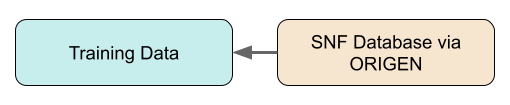
\includegraphics[width=0.7\linewidth]{./chapters/method/methodology1.png}
  \caption{First portion of the flowchart from Figure \ref{fig:method} being 
           described in this section.}
\end{figure}

Of interest to an entity trying to create a weapon is partially irradiated fuel
if they have plutonium separations capabilities or any radioactive substance in
the case of a dirty bomb. Thus, this work focuses on \gls{SNF} from commercial
power reactors. Ideally, a large enough database of \gls{SNF} nuclide assays
would be able to be used for this work. Since that does not exist, the 
database will be simulated via \gls{ORIGEN-ARP} \cite{origen, origenarp}.  

\subsubsection{Training Set Labels}
\label{sec:snflbls}

\begin{table}[!h]
  \centering
  \begin{subtable}{\linewidth}
    \centering
    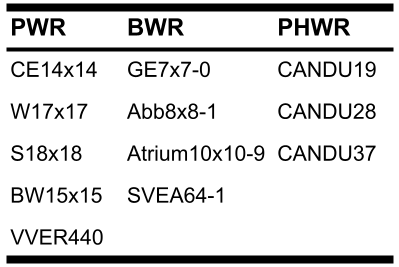
\includegraphics[width=0.5\linewidth]{./chapters/method/trainset4_Orxtrs.png}
    \caption{\gls{ORIGEN} designations for reactor technologies and fuel assembly design.}
    \label{tbl:rxtrtype}
    \vspace*{5mm}
  \end{subtable}
  \begin{subtable}{\linewidth}
    \centering
    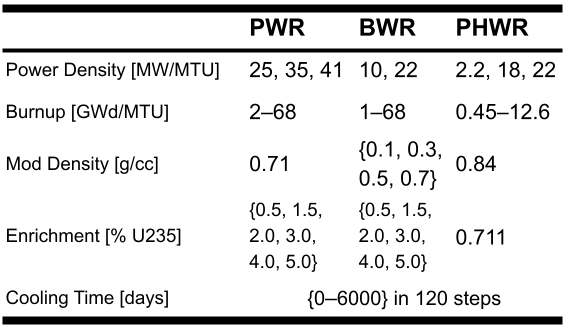
\includegraphics[width=0.75\linewidth]{./chapters/method/trainset4_inputs.png}
    \caption{Simulation parameters for \gls{ORIGEN} input files.}
    \label{tbl:rxtrparam}
  \end{subtable}%
  \caption{Training set database design using the \gls{SFCOMPO} database as guidance. \cite{sfcompo}}
  \label{tbl:train}
\end{table}

The design of the training set is dependent on a number of factors.  First, it
must have a sufficient number of burnup sets and time since irradiation steps
to provide robust prediction. This is decided upon by maximizing the steps for
both parameters, while balancing the computational limitations of a large
training set. Through previous experience, an approximate upper limit would be
somewhere around $1e6$ database entries for the specific calculations being
done in this work.

Secondly, the training set must represent what exists in the real world. This
was accomplished by studying the spread of parameters in the \gls{SFCOMPO}
database \cite{sfcompo}.  To ensure this, a variety of reactor types and
assembly designs were included, listed in Table \ref{tbl:rxtrtype}. Table
\ref{tbl:rxtrparam} lists the rest of the simulation inputs. These include not
only the labels of prediction interest, \gls{U235} enrichment, burnup, and time
since irradiation, but also other important simulation input parameters such as
the reactor power density and the moderator density.  (Water is both the
moderator and coolant in all simulated reactor types.)

\todo[inline]{add section reference} The third factor influencing database
design is ensuring ideal \gls{ML} algorithm performance.  As mentioned in
Section X, many algorithms are developed with the assumption that the training
set will be \acrfull{i.i.d.}.  This is important so that the model does not
overvalue or overfit a certain area in the training space. With the training
set design, there are predetermined values for enrichment, burnup, and time
since irradiation.  While there are $21-28$ burnup steps (depending on the
reactor type) and 120 cooling time steps, there are only 6 values for
enrichment. This creates the risk that the algorithm will end up being unable
to generalize outside of those discrete values. Therefore, the burnup steps and
time steps are perturbed randomly in a range that is $\pm10\%$ and $\pm30\%$
from the originally defined values, respectively.  The enrichment also gets
perturbed by $\pm10\%$, and not more because the cross-section libraries in
\gls{ORIGEN-ARP} are pre-calculated for those enrichment values, so deviating
too far from them would result in inaccurate \gls{SNF} simulations. The power
densities and moderator densities were kept at the values defined in Table
\ref{tbl:rxtrparam}.  The resulting training set is $5e5$.  Figure
\ref{fig:trainhist} visualizes the somewhat even distribution of the burnup and
cooling time parameters, and shows the lack of even distribution of the
enrichment parameter through a combination of scatter plots and histograms.
Note that there are many more \gls{BWR}s present in the histograms because of
the multiple moderator densities simulated (see Table \ref{tbl:rxtrparam})
\todo[inline]{update trainset size}

\begin{figure}[!htb]
  \makebox[\textwidth][c]{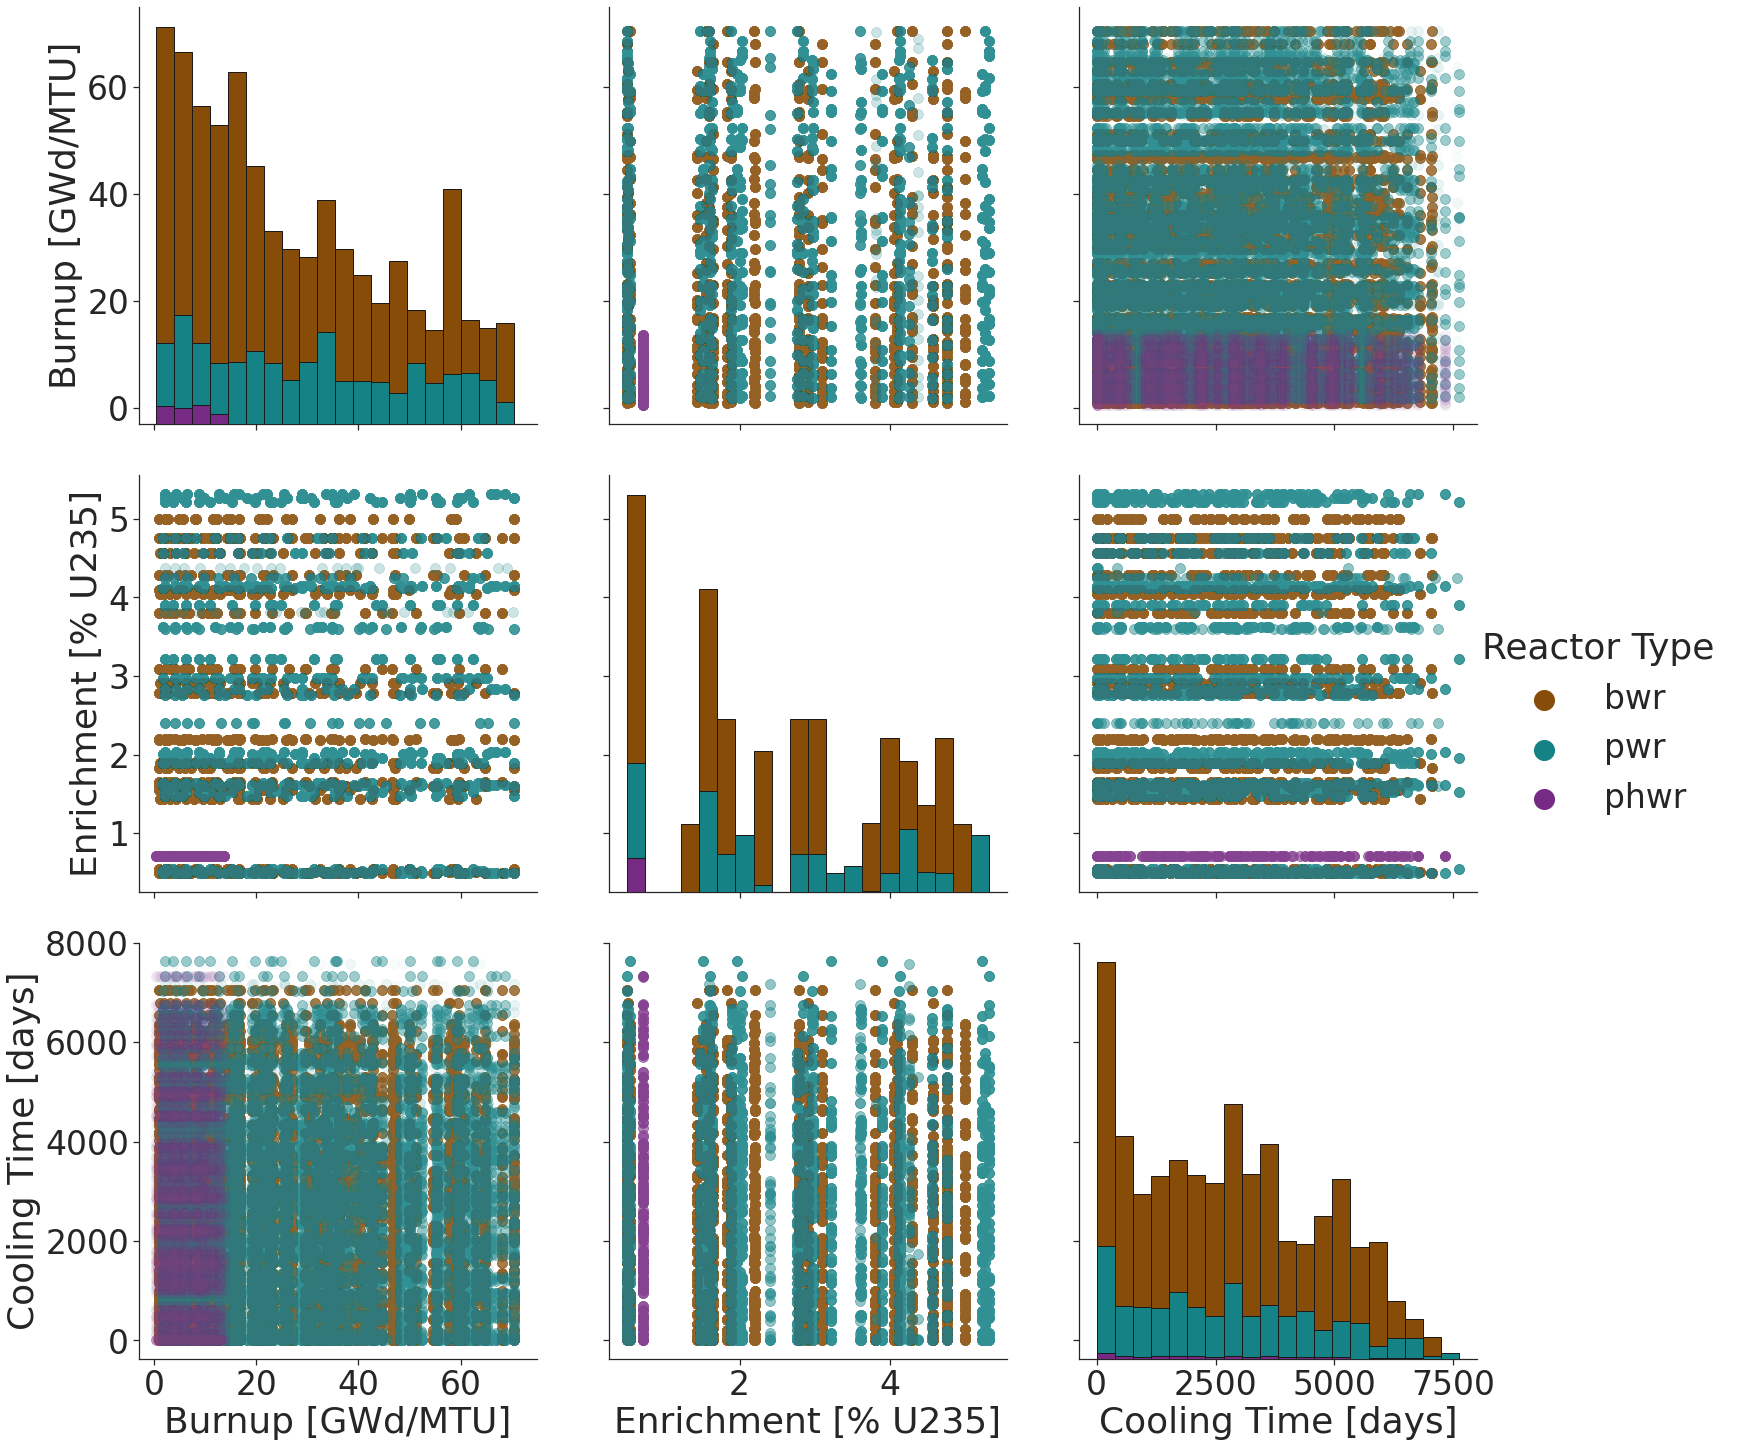
\includegraphics[width=\linewidth]{./chapters/method/histogram_scatter_trainset_viz.png}}
  \caption{A combination of histograms and scatter plots to visualize the 
           distribution of prediction labels in the training set.
           \textbf{\Large fix the histogram figure, this is a placeholder}}
  \label{fig:trainhist}
\end{figure}

\subsubsection{Training Set Features}
\label{sec:snffeats}

\todo[inline]{need to outline two exmpts before this. Writing this with that
assumption.} The other design decision regarding the training set is related to
which nuclides to track, i.e., the features.  For the first experiment, nuclide
masses are necessary, and the most common measurements in \gls{SFCOMPO} guide
the list of nuclides tracked.  In the second experiment, activities of
radionuclides are necessary to calculate gamma spectra from these values.

The first experiment with the 29 nuclide masses listed in Table
\ref{tbl:nucmass} was designed with the following reasons in mind.  First, the
units in mass is to represent the scenario of "perfect knowledge", where a full
assay is done via mass spectrometry techniques.  Second, this is to have the
training set units convertable to those present in the external, real-world
test set: the \gls{SFCOMPO} database.  The \gls{ORIGEN} simulations output the
nuclide masses in $grams$, and they are converted to the units of
\textit{milligrams per gram of initial uranium}, $mg/gU_i$, when the models are
externally tested against \gls{SFCOMPO}. Lastly, the 29 nuclides chosen were
based on the presence of measurements in \gls{SFCOMPO}, where these were
present in at least 100 of the samples in the database.  The test set is
described in more detail in Section \ref{sec:eval}.

\begin{table}[!h]
  \centering
  \begin{subtable}{\linewidth}
    \centering
    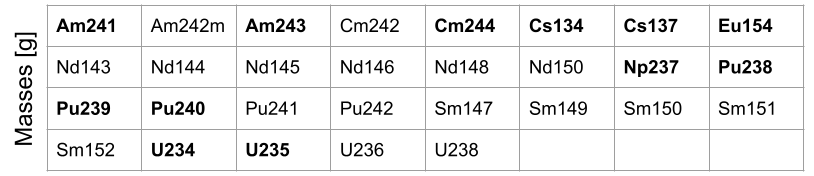
\includegraphics[width=\linewidth]{./chapters/method/nucmass_feats.png}
    \caption{Set of features saved for the first experiment, nuclide masses 
             measured in $grams$. The bold nuclide masses overlap with the 
             nuclides in \ref{tbl:nucacts}.}
    \label{tbl:nucmass}
    \vspace*{5mm}
  \end{subtable}
  \begin{subtable}{\linewidth}
    \centering
    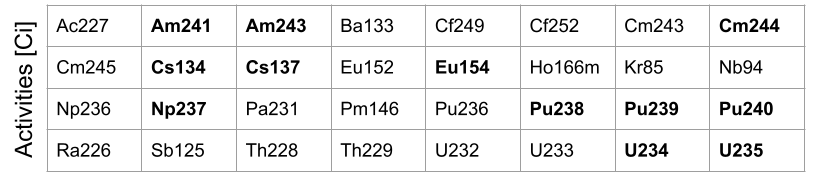
\includegraphics[width=\linewidth]{./chapters/method/nucacts_feats.png}
    \caption{Set of features saved for the second experiment, nuclide activities
             measured in $Curies$. The bold nuclide activities overlap with the 
             nuclides in \ref{tbl:nucmass}.}
    \label{tbl:nucacts}
  \end{subtable}%
  \caption{Two sets of features saved from the same simulation inputs for the 
           two main experiments in this work.}
  \label{tbl:nucfeats}
\end{table}

The second feature set with the 32 nuclide activities listed in Table
\ref{tbl:nucacts} was designed with the following reasons in mind. First,
nuclide activities are the most straightforward units to use for application to
the \gls{DRF} in the \gls{GADRAS} tool for the second experiment. This process
is used to obtain gamma spectra for each \gls{SNF} entry in the database, which
is detailed in \ref{sec:inforeduc}.  Second, these specific nuclides were
chosen because they fulfill four steps of filtering:
\begin{enumerate}
  \item They exist in the 196-long radionuclide list in \gls{GADRAS}.
  \item They have an activity above $1e-7\:Ci$ (cutoff chosen to filter out
  nuclides that are unlikely to produce gamma energy peaks).
  \item They have a half-life longer than $1\:year$ (cutoff chosen based on
  maximum cooling time of $16\:years$).
  \item They have at least one gamma energy line above $200\:keV$ (cutoff
  chosen based on low-energy gamma energy peaks being difficult to discern in
  some detectors).
\end{enumerate}

\subsubsection{Simulation Fidelity}
\label{sec:fidelity}

\todo[inline]{This section needs to be written about \gls{ORIGEN-ARP}
validation and maybe some nuclides that are known to perform poorly from ARP
sims. Can show a generic example from one of my sources, and or an example of
trying to match an \gls{ORIGEN-ARP} simulation to an \gls{SFCOMPO} entry.}

\subsection{Information Reduction}
\label{sec:inforeduc}

\begin{figure}[H]
  \centering
  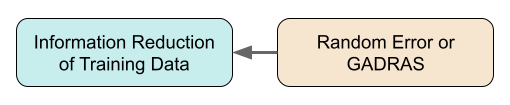
\includegraphics[width=0.7\linewidth]{./chapters/method/methodology2.png}
  \caption{Second portion of the flowchart from Figure \ref{fig:method} being 
           described in this section.}
\end{figure}

Since the overall goal of this project is to determine how much information to
what quality is needed to train an \gls{ML} model that can provide \gls{SNF}
attribution, there will be an information reduction manipulation applied to the
training data set. The first experiment 

This study evaluates
the impact of randomly introduced error on the ability of the algorithms to
correctly predict the burnup. 

The three algorithms will be evaluated with error applied to each nuclide
vector in the training set.  A maximum error ranging from $0 - 10\%$ is chosen
for each round of training, and a random error within the range of $[1-E_{max},
1+E_{max}]$ is applied to each component of the nuclide vector.

However, error in a nuclide vector is not random, in fact it is systematic and
dependent on a number of known sources of uncertainty. The next study will
introduce error by limiting the nuclides to only those that can be measured
with a gamma spectrometer. Although this is initially done using the
availability of gamma energies in \gls{ORIGEN}, \gls{GADRAS} can provide more
\gls{DRF}s to further reduce information given to the algorithm.

Next, this work will expand upon the previous work.  The first future step is a
different information reduction technique using gamma energies from \gls{SNF}
nuclide recipes.  Following this, one could apply a \gls{DRF} that calculates
various spectra based on the types of gamma detectors available to the
forensics community 

Gamma spec details: 1g of material, 600 sec measurement, 6 detectors w decreasing 
energy resolution, no background, non-zero source age (20 min -- check on this).
Using DetectorSetups.txt: make table w detectors, their nchannels, height and distance,
and other relevant info from the detector dir in gadras\_run\_directory.
